%SI 2014-09-05

\documentclass{article}

\usepackage[T1]{fontenc}
\usepackage[utf8]{inputenc}
\usepackage[swedish]{babel}
\usepackage{fullpage}
\usepackage{amssymb}
\usepackage{bussproofs}
\usepackage{amsmath}
\usepackage{wrapfig}
\usepackage{float}
\usepackage{graphicx}
\usepackage{verbatim}
\usepackage{tikz}
\let\emptyset\varnothing


\title{Supplemental Instructions}
\date{
      %Place date here!
     }

\begin{document}
\maketitle


\section*{1}
Om vi kikar på integralen som ges på s. 368: $\int_a^b f(x) dx$, så är: \\
a = 0, b = $\pi$, $f(x) = sin(x)$, $x_i = a+ih$\\\\

\noindent
a) \\
\noindent
$n = 10 \Rightarrow h = \frac{b-a}{n} = \frac{\pi}{10}$ och 

\begin{tabular}{l|l*{6}{c}} \\
$i$     & 0 & 1 & 2 & 3 & ...  & 9 & 10 \\
\hline
$x_i$   & 0 & $\frac{\pi}{10}$ & $\frac{2 \pi}{10}$ & $\frac{3 \pi}{10}$ & 
        ... & $\frac{9 \pi}{10}$ & $\frac{10 \pi}{10}$  \\
        [5pt]
$f_i$   & $sin(0)$ & $sin(\frac{\pi}{10})$ & $sin(\frac{2 \pi}{10})$ & 
        $sin(\frac{3 \pi}{10})$ & ... & $sin(\frac{9 \pi}{10})$ & 
        $sin(\frac{10 \pi}{10})$ \\
\end{tabular}\\\\
[20pt]
$\int_0^{\pi} sin(x) dx \approx \frac{h}{2}[f_0 + 2f_1 + 2f_2 + 2f_3 + ... + 2f_9 + f_{10}]
 = 1.983 523 538$\\\\
Error = $0.824\%$\\\\
\noindent
b) \\
\noindent
$n = 20 \Rightarrow h = \frac{\pi}{20}$\\\\
$\int_0^{\pi} sin(x) dx \approx \frac{h}{2}[f_0 + 2f_1 + 2f_2 + 2f_3 + ... + 2f_{19} + f_{20}]
= 1.995 885 973$\\\\
Error = $0.206\%$


\section*{2}
$\frac{\pi}{5}$ cu. units

\section*{3}
\begin{itemize}
	\item[a) ] $y = \frac{4}{3} \> x$, där x går från 0 till 3. \\
			 Här får vi en vanlig triangel med basen 3 och höjden 4. Längden blir således 5, enl pythagoras. 
			 
	\item[b) ] 	$y = \frac{2}{3} (x-1)^{ \frac{3}{2} }$, där x går från 0 till 4 \\
				Här måste vi använda längdformeln. 
				$ds = \sqrt{1 + f'(x)^2}$ \\
				$ds = \sqrt{1 + x-1} $ \\
				$ds = \sqrt{x} $ \\
				$L = \int_{0}^{4} ds = \int_{0}^{4} \sqrt{x} dx $ \\
				$L =  2/3 ( 4^{3/2} - 0^{3/2} ) = 2/3 * 8 = 16/3 $
\end{itemize}


\section*{4}
Volymen = $\int_0^2 \pi(x(2-x)^2)dx$\\\\
$$\pi \int_0^2 x^2(4-4x+x^2)dx = 
\pi \int_0^2 4x^2-4x^3+x^4 = 
\pi \begin{bmatrix} \frac{4x^3}{3} - \frac{4x^4}{4} + \frac{x^5}{5} \end{bmatrix}_0^2 = 
\pi (\frac{3^2}{2} - 16 + \frac{3^2}{5}) = 
16 \pi(\frac{10}{15} - \frac{15}{15} + \frac{6}{15}) = 
\frac{16 \pi}{15}$$

\section*{5}
\begin{wrapfigure}{R}{0.4\textwidth}
\centering
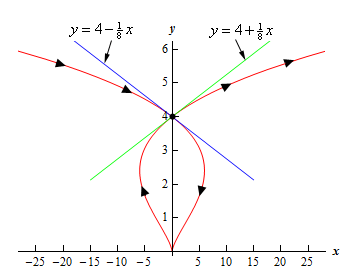
\includegraphics[width=0.5\textwidth]{curvesol}
\end{wrapfigure}
$x = t^5 - 4t^3 = t^3 (t^2-4)$   \\
$y = t^2$ \\ \\ 
Vi vill ha $\frac{dy}{dx}$ vilket är lika med $\frac{dy}{dt} \Big/  \frac{dx}{dt} $. \\
$\frac{dy}{dt} = 2t$ och $\frac{dx}{dt} = 5t^4 - 12t^2$. \\ \\ 
$\frac{dy}{dx} = \frac{2t}{5t^4 - 12t^2} = \frac{2}{5t^3 - 12t}$ . \\ \\ 
Nu vill vi hitta $t$ så att $x(t) = 0$ och $y(t) = 4$  \\
$x(t) = 0 \implies t = 0, -2, 2$, \quad
$y(t) = 4 \implies t = -2, 2$. \\
Här har vi -2 och 2 som är gemensamma. Beräkna nu $\frac{dy}{dx}$. \\
$t = -2 \implies \frac{dy}{dx} = \frac{2}{5(-2)^3 - 12(-2)} = -\frac{1}{8}$ \\
$t =  2 \implies \frac{dy}{dx} = \frac{2}{5(2)^3  - 12(2)}  = \frac{1}{8}$ \\
Så för $y = kx + m$ så får vi \\ 
$y_1 = -\frac{1}{8}x + 4$ och $y_2 = \frac{1}{8}x + 4$. 









\end{document}
